% Page: Reliability
% sources/stat2003/chapters/prob-07-reliability.qmd
% The bridge that the page says cannot be drawn as a series-parallel graph.
% Side paths 1-4 and 2-5, cross link 3. The system works when the left
% terminal is connected to the right through working components.
\documentclass[border=6pt]{standalone}
\usepackage[T1]{fontenc}
\usepackage{lmodern}
\usepackage{amsmath,amssymb}
\usepackage{tikz}
\usetikzlibrary{calc}
\definecolor{ink}{HTML}{1F2430}
\definecolor{statblue}{HTML}{174A7E}
\definecolor{soft}{HTML}{F4F6F8}
\definecolor{grey}{HTML}{5E6A75}
\begin{document}
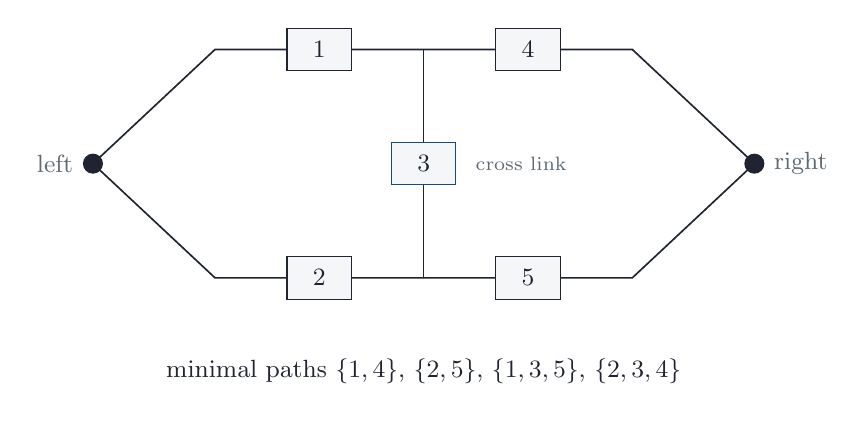
\begin{tikzpicture}[
  font=\small,
  every node/.style={text=ink},
  comp/.style={draw=ink, thin, fill=soft, minimum width=8.2mm, minimum height=5.4mm, inner sep=0pt},
  wire/.style={ink, line width=0.6pt},
  terminal/.style={circle, draw=ink, fill=ink, inner sep=0pt, minimum size=2.4mm},
]
  \coordinate (S) at (0,0);
  \coordinate (T) at (8.4,0);
  \coordinate (UL) at (1.55,1.45);
  \coordinate (UM) at (4.20,1.45);
  \coordinate (UR) at (6.85,1.45);
  \coordinate (LL) at (1.55,-1.45);
  \coordinate (LM) at (4.20,-1.45);
  \coordinate (LR) at (6.85,-1.45);

  \draw[wire] (S) -- (UL) -- (UM) -- (UR) -- (T);
  \draw[wire] (S) -- (LL) -- (LM) -- (LR) -- (T);
  \draw[wire] (UM) -- (LM);

  \node[comp] (c1) at ($(UL)!0.5!(UM)$) {$1$};
  \node[comp] (c4) at ($(UM)!0.5!(UR)$) {$4$};
  \node[comp] (c2) at ($(LL)!0.5!(LM)$) {$2$};
  \node[comp] (c5) at ($(LM)!0.5!(LR)$) {$5$};
  \node[comp, draw=statblue] (c3) at ($(UM)!0.5!(LM)$) {$3$};

  \node[terminal, label={[grey]left:left}] at (S) {};
  \node[terminal, label={[grey]right:right}] at (T) {};
  \node[font=\scriptsize, grey, anchor=west] at ($(c3.east)+(0.12,0)$) {cross link};

  \node[anchor=north, align=center, font=\small] at ($(S)!0.5!(T)+(0,-2.35)$)
    {minimal paths $\{1,4\}$, $\{2,5\}$, $\{1,3,5\}$, $\{2,3,4\}$};
\end{tikzpicture}
\end{document}
